\chapter{Interfacce}

Per realizzare le pagine sono stati usati \emph{HTML 5} e \emph{Bootstrap}.\\
Gli elementi di personalizzazione, come il nome utente nella navbar una volta autenticati o il meteo
in tempo reale delle città salvate tra i preferiti, sono inseriti utilizzando \emph{EJS}.

\section{Index.ejs}

\begin{figure}[ht]
    \centering
    \resizebox{\textwidth}{!}{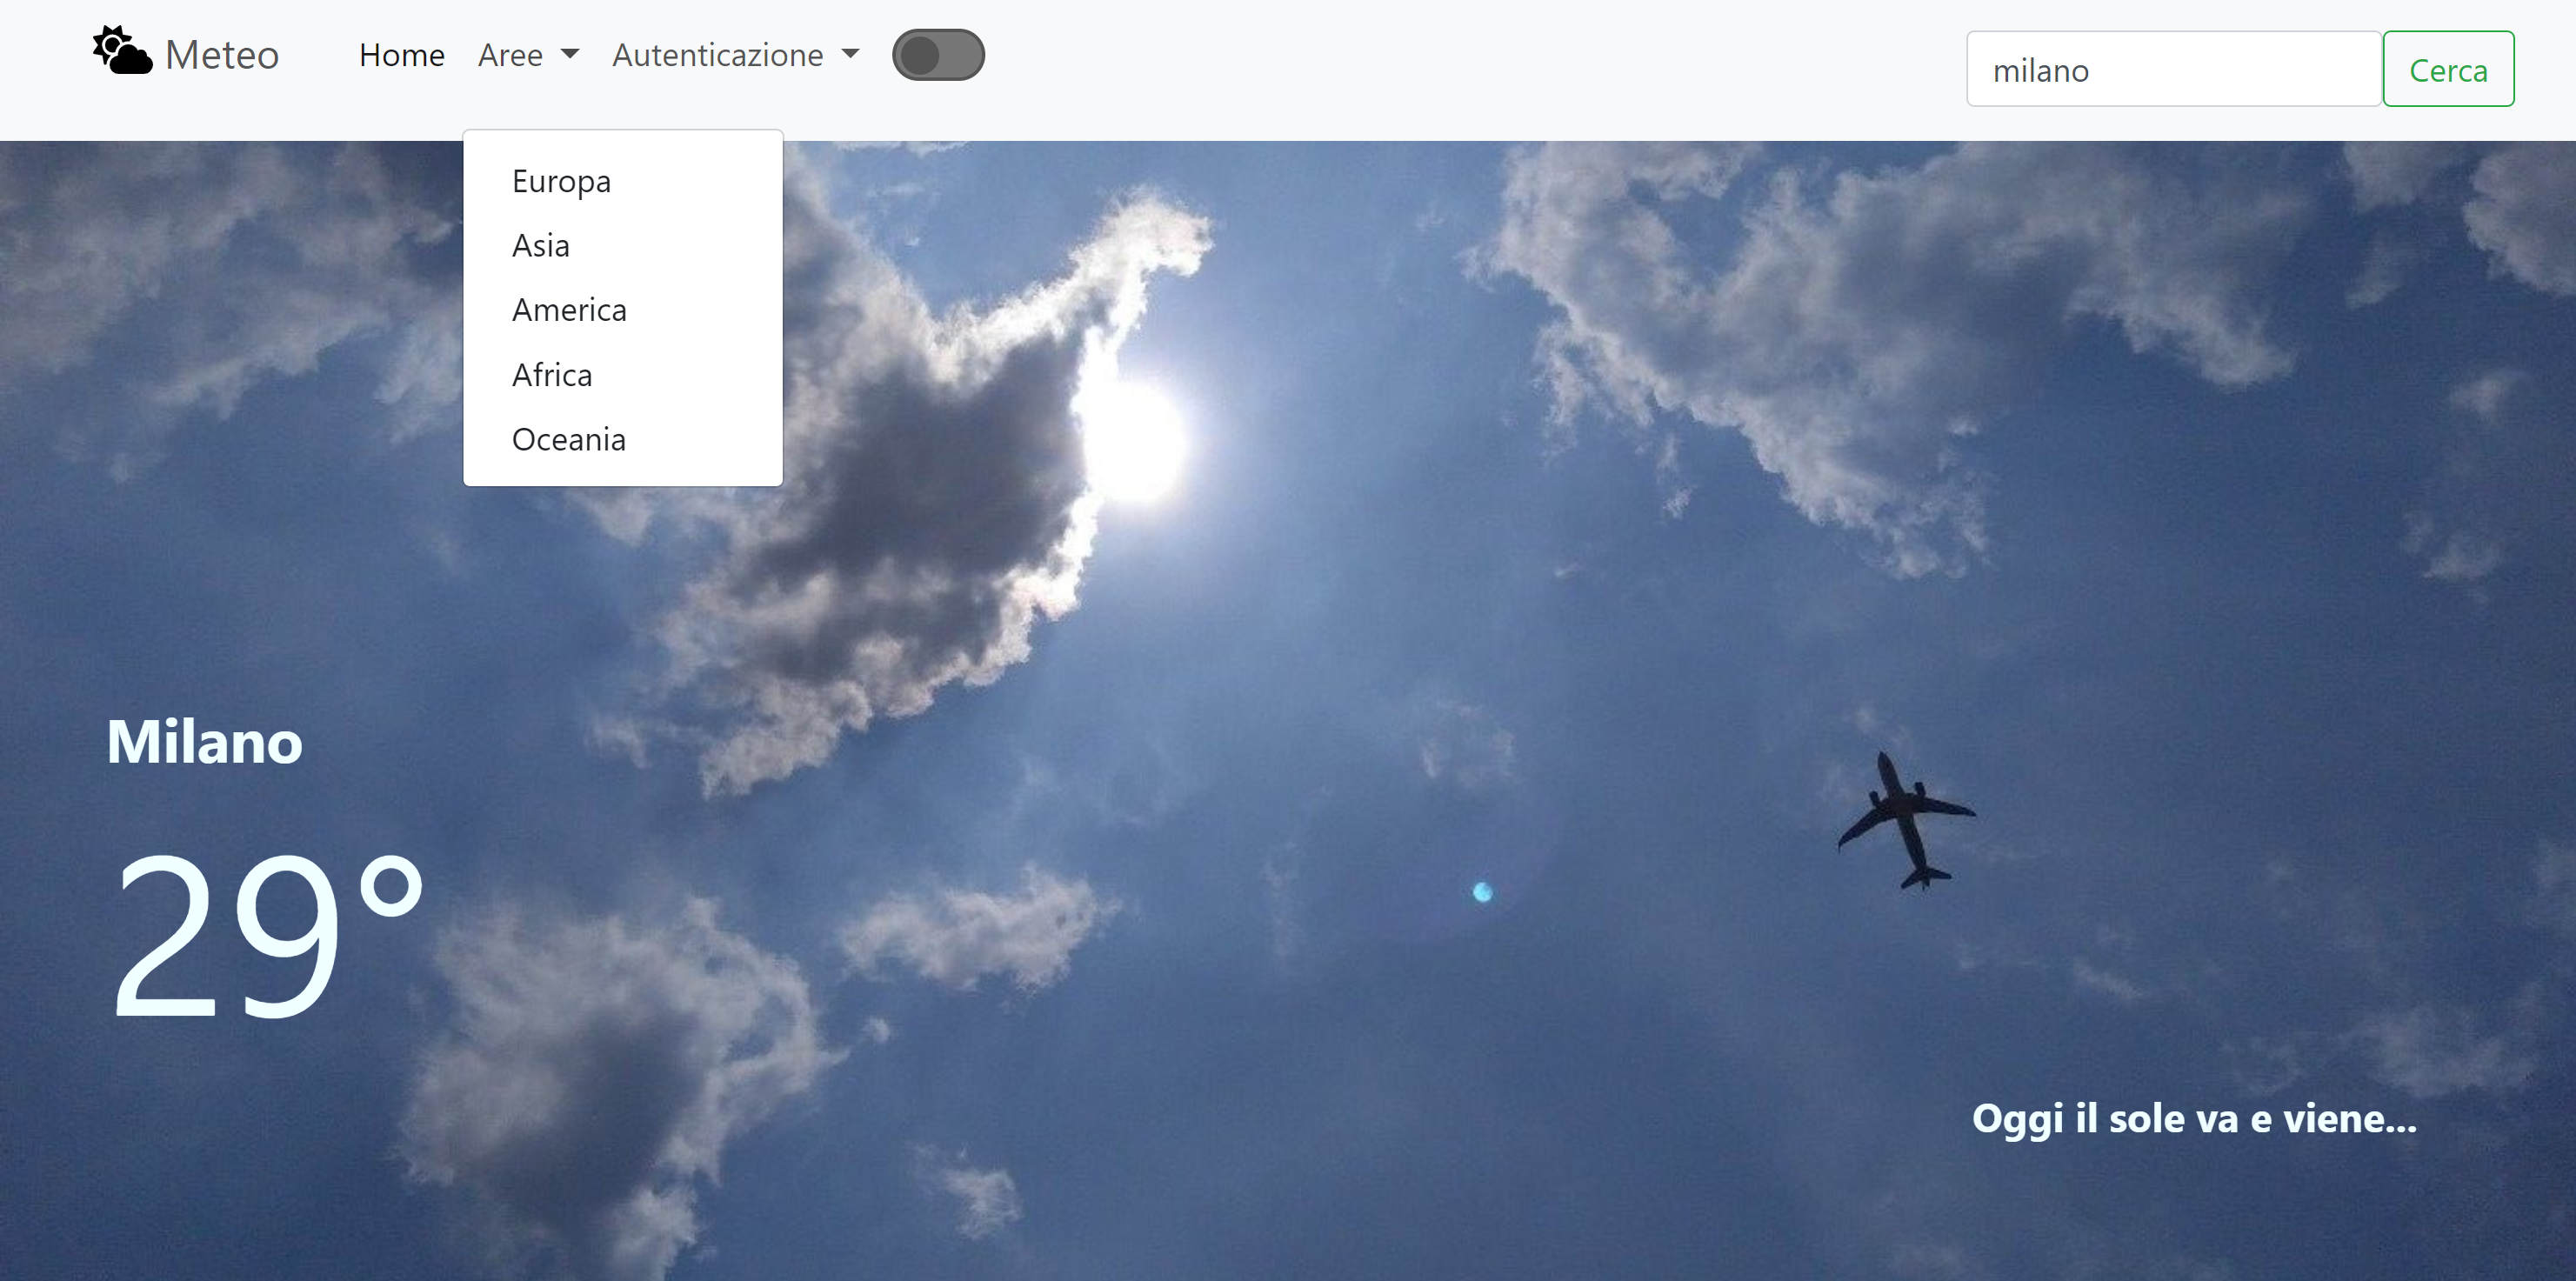
\includegraphics{img/indexSopra.png}}
    \caption{Metà superiore dell'home page}
\end{figure}

Nella parte superiore dell'index come prima cosa troviamo una navbar semplice con elementi completamente intuitivi: a partire da sinistra si ha il nome e il logo dell'applicazione,
e il tasto home; grazie al menù a tendina \emph{Aree} è possibile navigare per aree geografiche (i continenti) e cercare informazioni sulle città relative ad esse; cliccando invece sul menù \emph{Autenticazione}
l'utente può accedervi o registrarsi; a seguito del login, questo menù viene sostituito con un altro per poter effettuare il logout e per poter accedere all'area personale, dove sono salvate le città
preferite dall'utente e dove quest'ultimo può cambiare le informazioni di accesso. \\
Sempre sulla navbar troviamo un toggle che dà la possibilità all'utente di cambiare la modalità di visualizzazione,
\emph{light mode} o \emph{dark mode}, a seconda della sua preferenza. Sulla destra troviamo invece una barra di ricerca.

\vspace{5mm}

Al di sotto della navbar troviamo un'immagine di copertina con le informazioni metereologiche relative alla città corrente, ottenute dalla geolocalizzazione e dall'apposita API;
questi dati, così come l'immagine di sfondo, vengono sostituite dalla città cercata nella barra di ricerca.

\begin{figure}[ht]
    \centering
    \resizebox{\textwidth}{!}{\includegraphics{img/indexLogged.png}}
    \caption{Metà inferiore dell'home page dopo aver effettuato il login}
\end{figure}

Superate le informazioni relative al servizio proposto, troviamo un'area apposita dove vengono visualizzati i dati metereologici delle città che sono state
salvate dall'utente nell'apposita area personale, a cui si può accedere solamente una volta effettuato il login (o registrazione). Motivo per il quale, in assenza di accesso verrà visualizzata una scritta
suggerendo all'utente di accedervi per poter visualizzare correttamente tutti i dati.

\begin{figure}[ht]
    \centering
    \resizebox{\textwidth}{!}{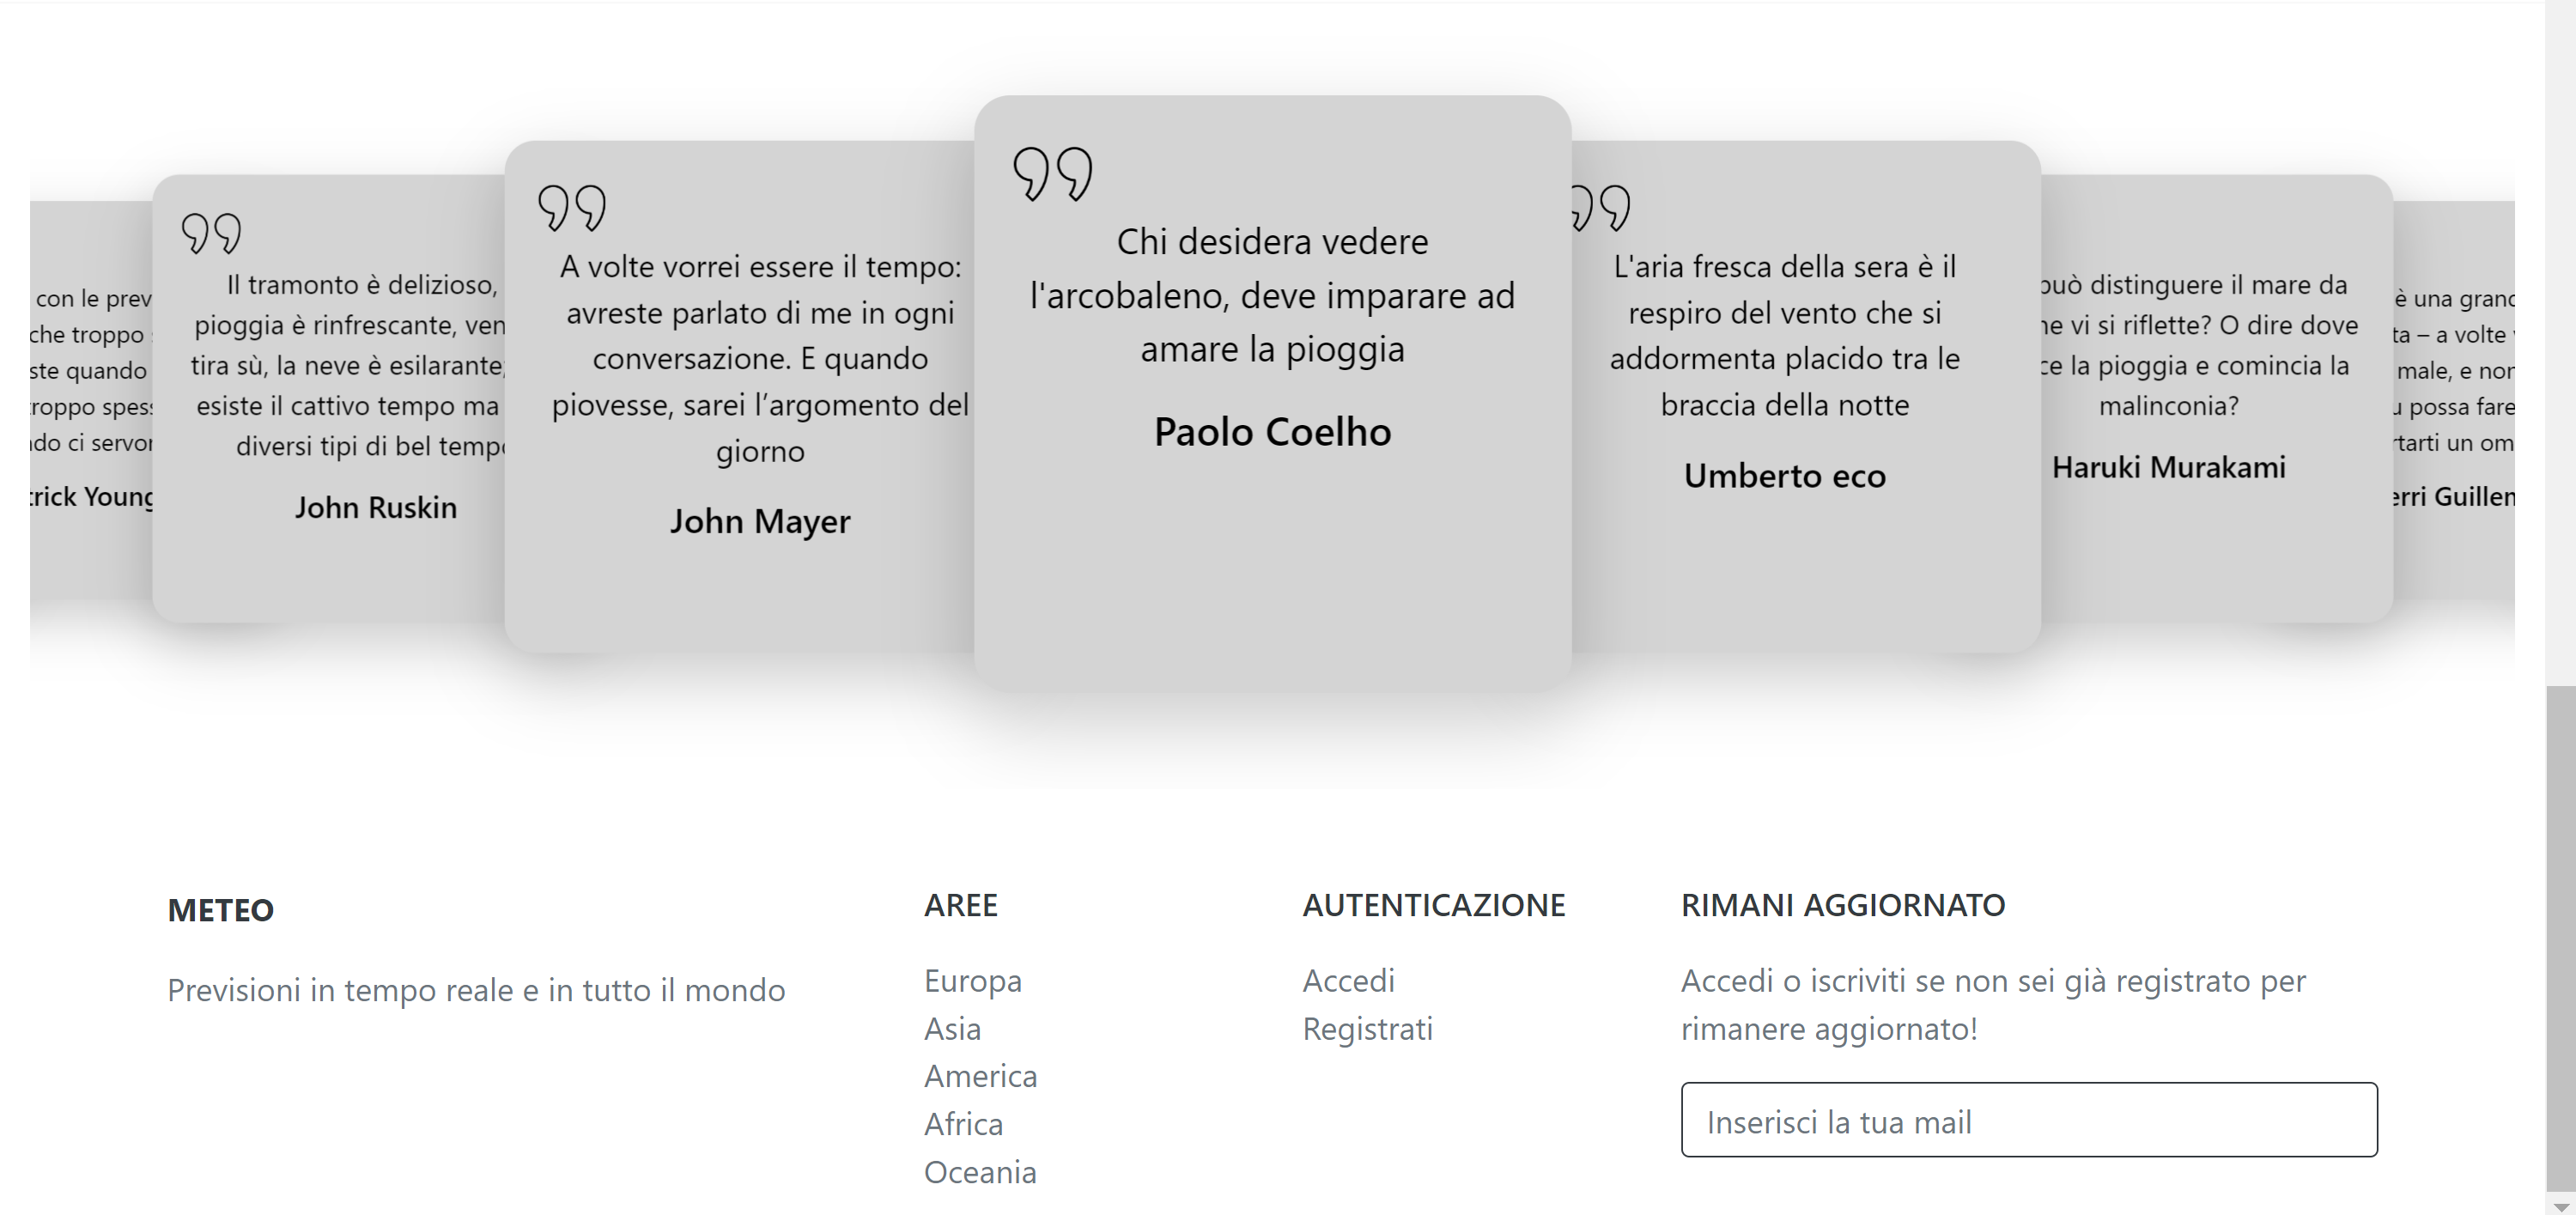
\includegraphics{img/swiperFooter.png}}
    \caption{Swiper con citazioni e footer}
\end{figure}

Oltre l'area dedicata alle città preferite, invece, troviamo uno slider ottenuto con \emph{Swiper API} in cui, scorrendo, si possono leggere alcune citazioni famose sul meteo.

\vspace{5mm}

In fondo ad ogni pagina dell'applicazione troviamo un footer con le informazioni di riepilogo e i riferimenti alle pagine del sito web, così come la possibilità di inserire la propria email per
rimanere aggiornato.

\newpage
\section{Aree}

\subsection{Area.ejs}

\section{Login e Registrazione}

\subsection{Login.ejs}

\begin{figure}[ht]
    \centering
    \resizebox{\textwidth}{!}{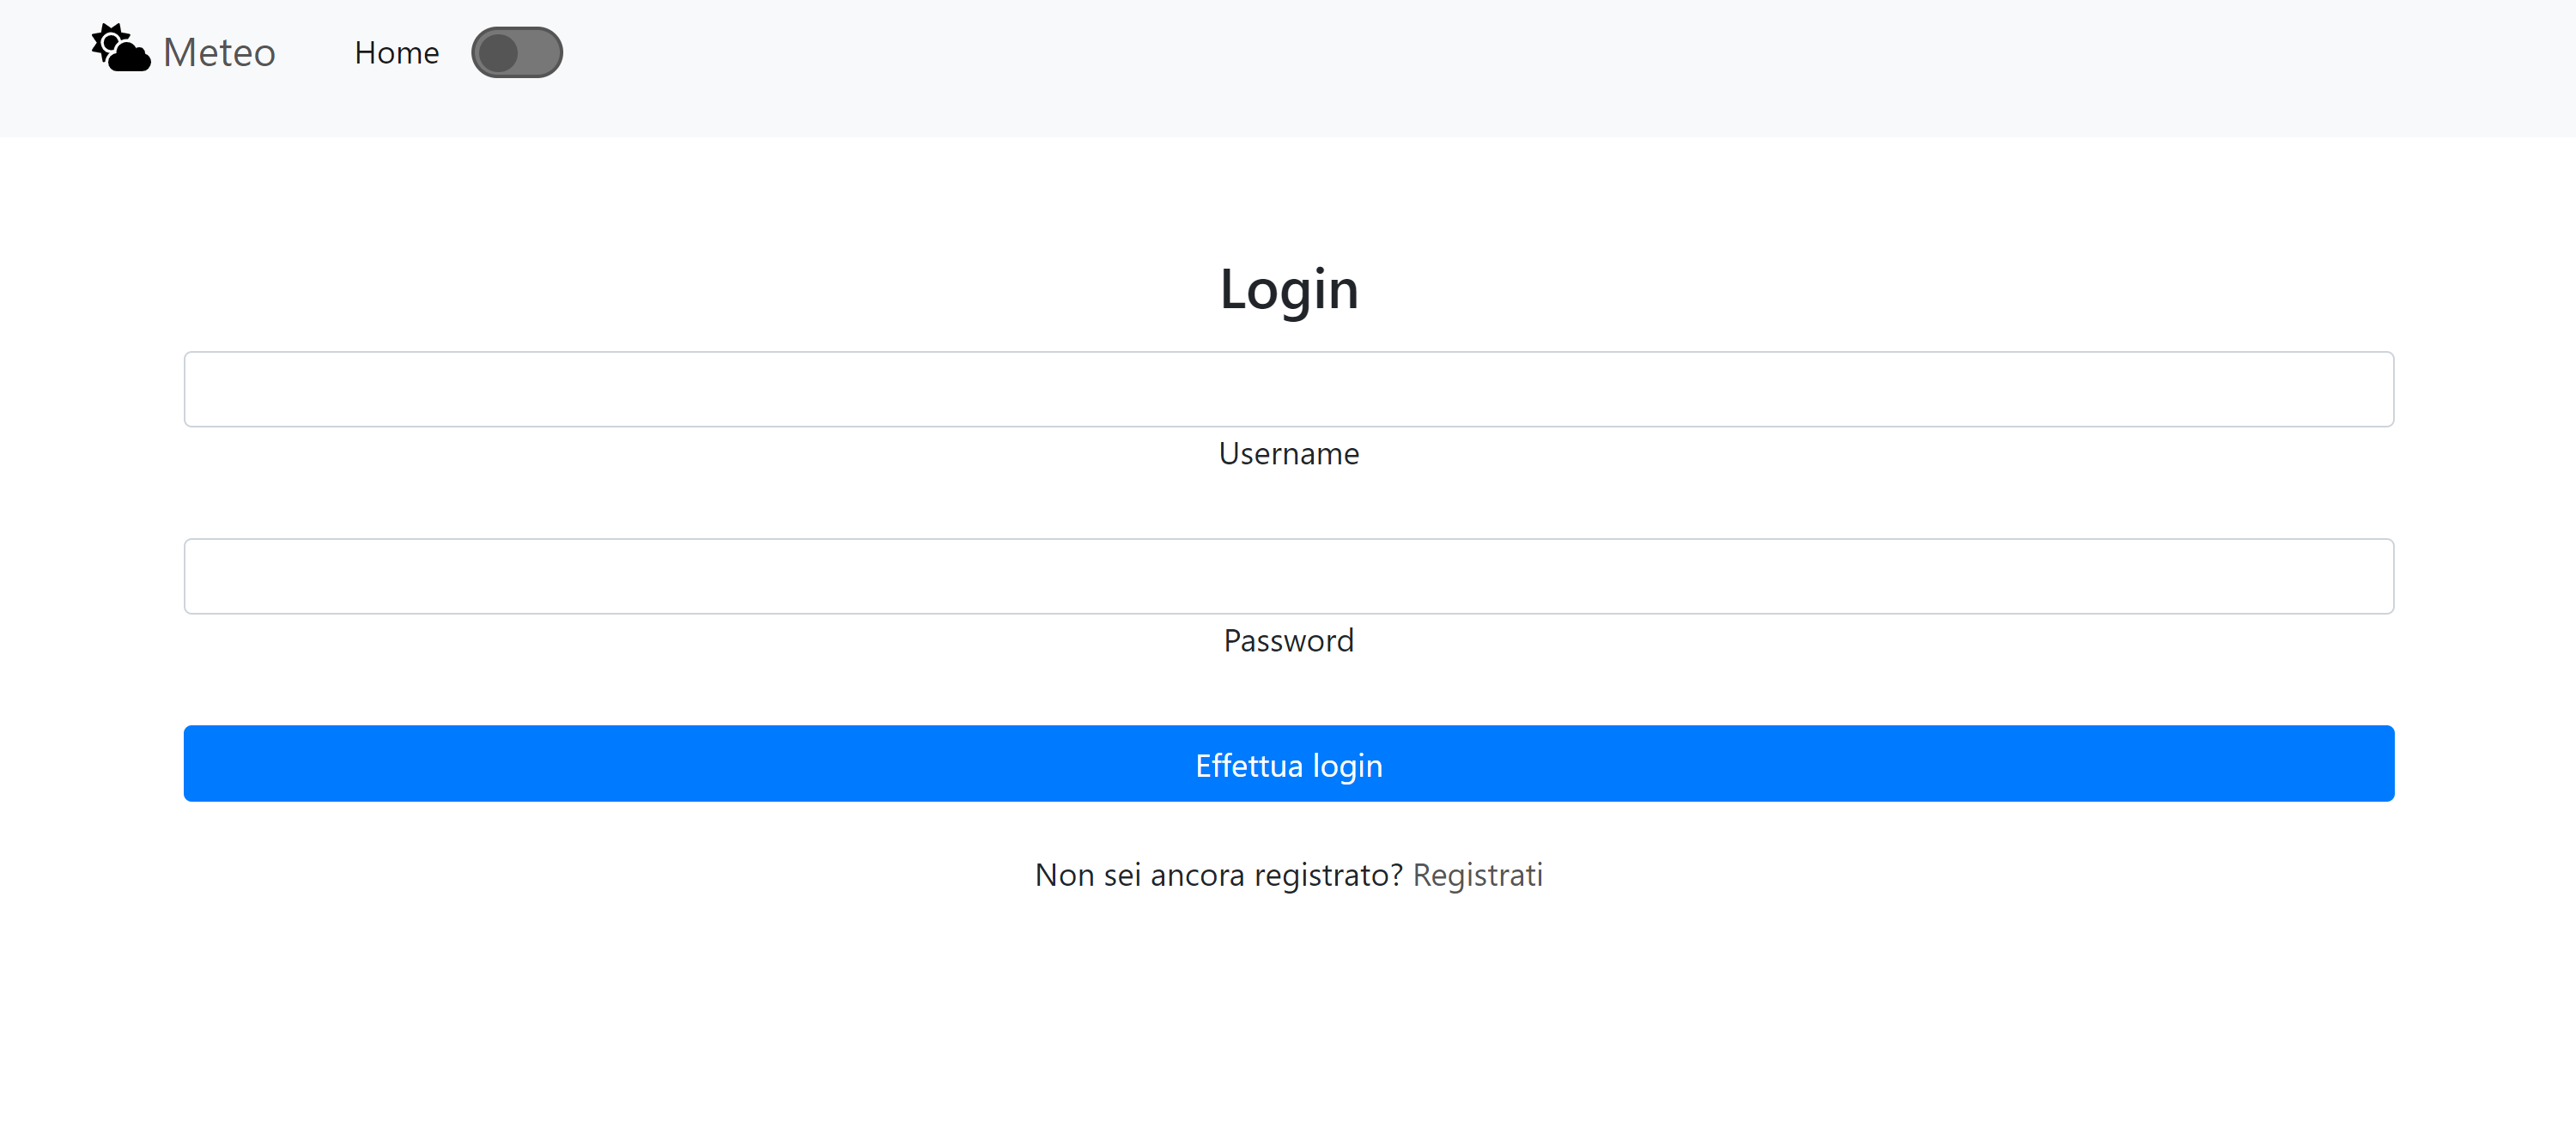
\includegraphics{img/login.png}}
    \caption{Pagina dedicata al login}
\end{figure}

Grazie a questa pagina è possibile effettuare il login nel caso si sia già registrati oppure di registrarsi attravero l'apposito
link al di sotto del form con le credenziali.\\
La navbar è semplificata in modo da rendere l'interfaccia meno dispersiva e permette unicamente di tornare alla home, gestire
la modalità di visualizzazione della pagina oppure cercare una città.

\newpage
\subsection{Registrazione.ejs}

\begin{figure}[ht]
    \centering
    \resizebox{\textwidth}{!}{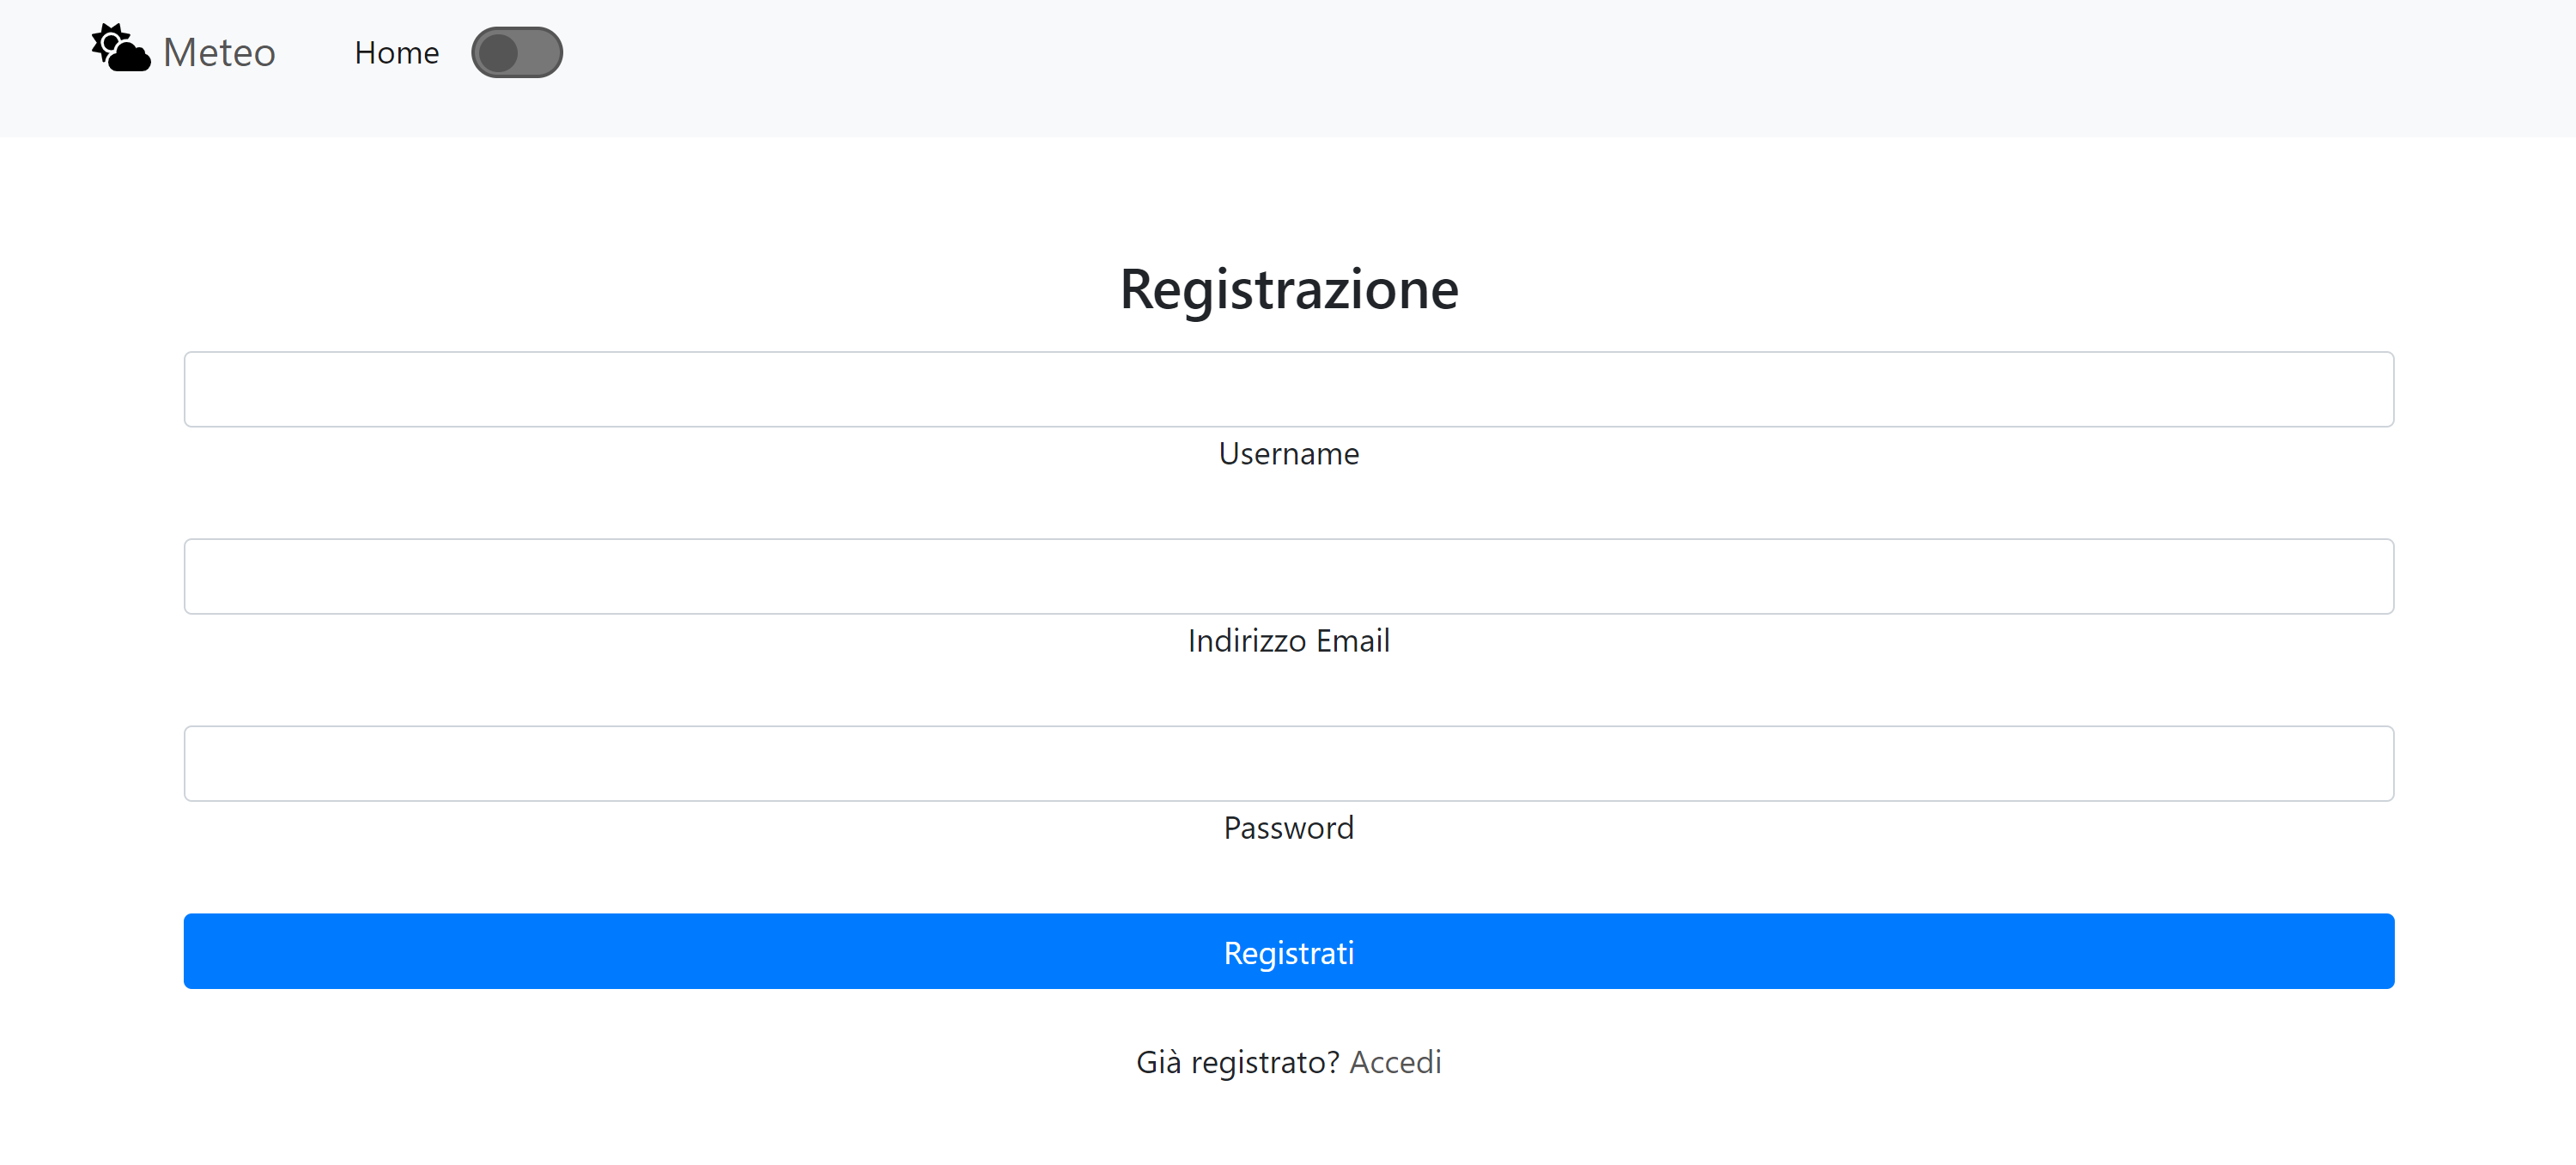
\includegraphics{img/registrazione.png}}
    \caption{Pagina dedicata alla registrazione}
\end{figure}

In questa pagina verranno richieste le credenziali usate in seguito per effettuare il login (email e password) e un nome utente.
Questi dati saranno modificabili in un secondo momento tramite l'area personale (\textbf{N.B.}: non è possibile avere più utenti con
la stessa mail e/o lo stesso username).\\

\vspace{5mm}

Se necessario, è possibile passare alla pagina di login tramite il link in basso.\\

\vspace{5mm}

La navbar è semplificata nella stessa maniera della pagina di login.

\newpage
\subsection{AreaPersonale.ejs}

\begin{figure}[ht]
    \centering
    \resizebox{\textwidth}{!}{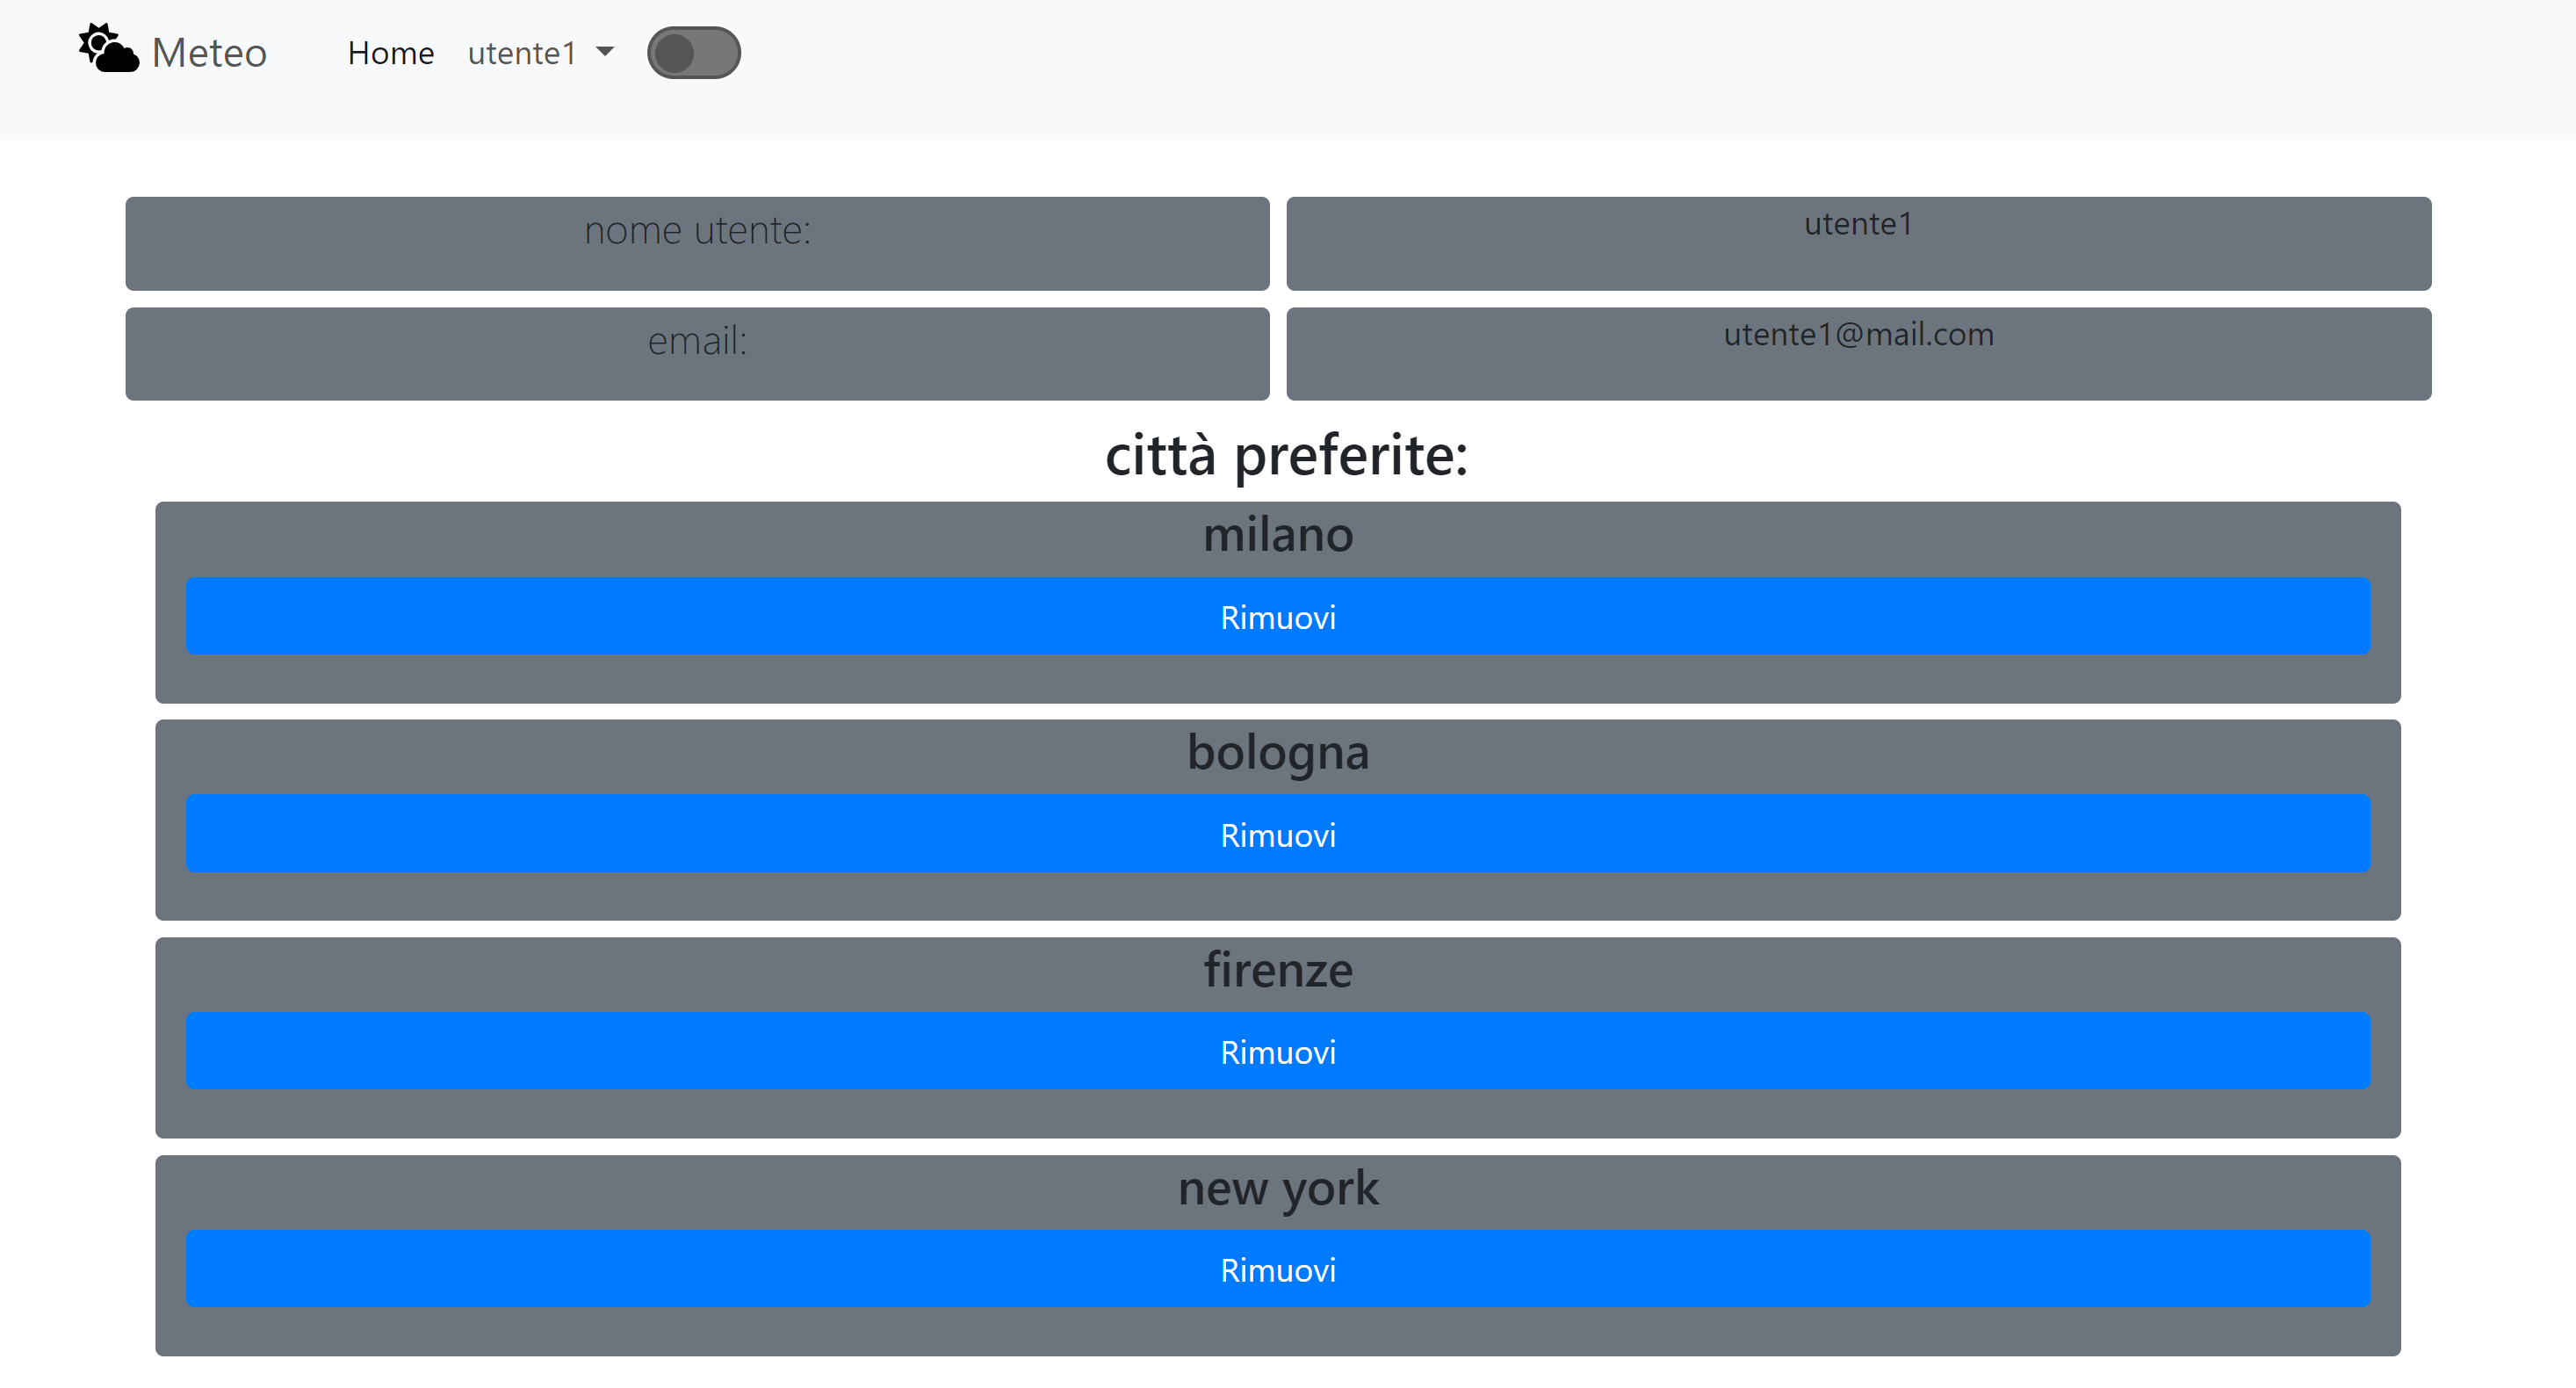
\includegraphics{img/areaPSopra.png}}
    \caption{Metà superiore della pagina dedicata all'area personale}
\end{figure}

Nella metà superiore della pagina troviamo una navbar analoga a quella presente nell'index a seguito del login.

\vspace{5mm}

Al di sotto di essa, abbiamo i dati relativi all'utente (username e email. la password non viene mostrata per ragioni di
sicurezza) e l'elenco delle città salvate tra i preferiti, se presenti.

\newpage
\begin{figure}[ht]
    \centering
    \resizebox{\textwidth}{!}{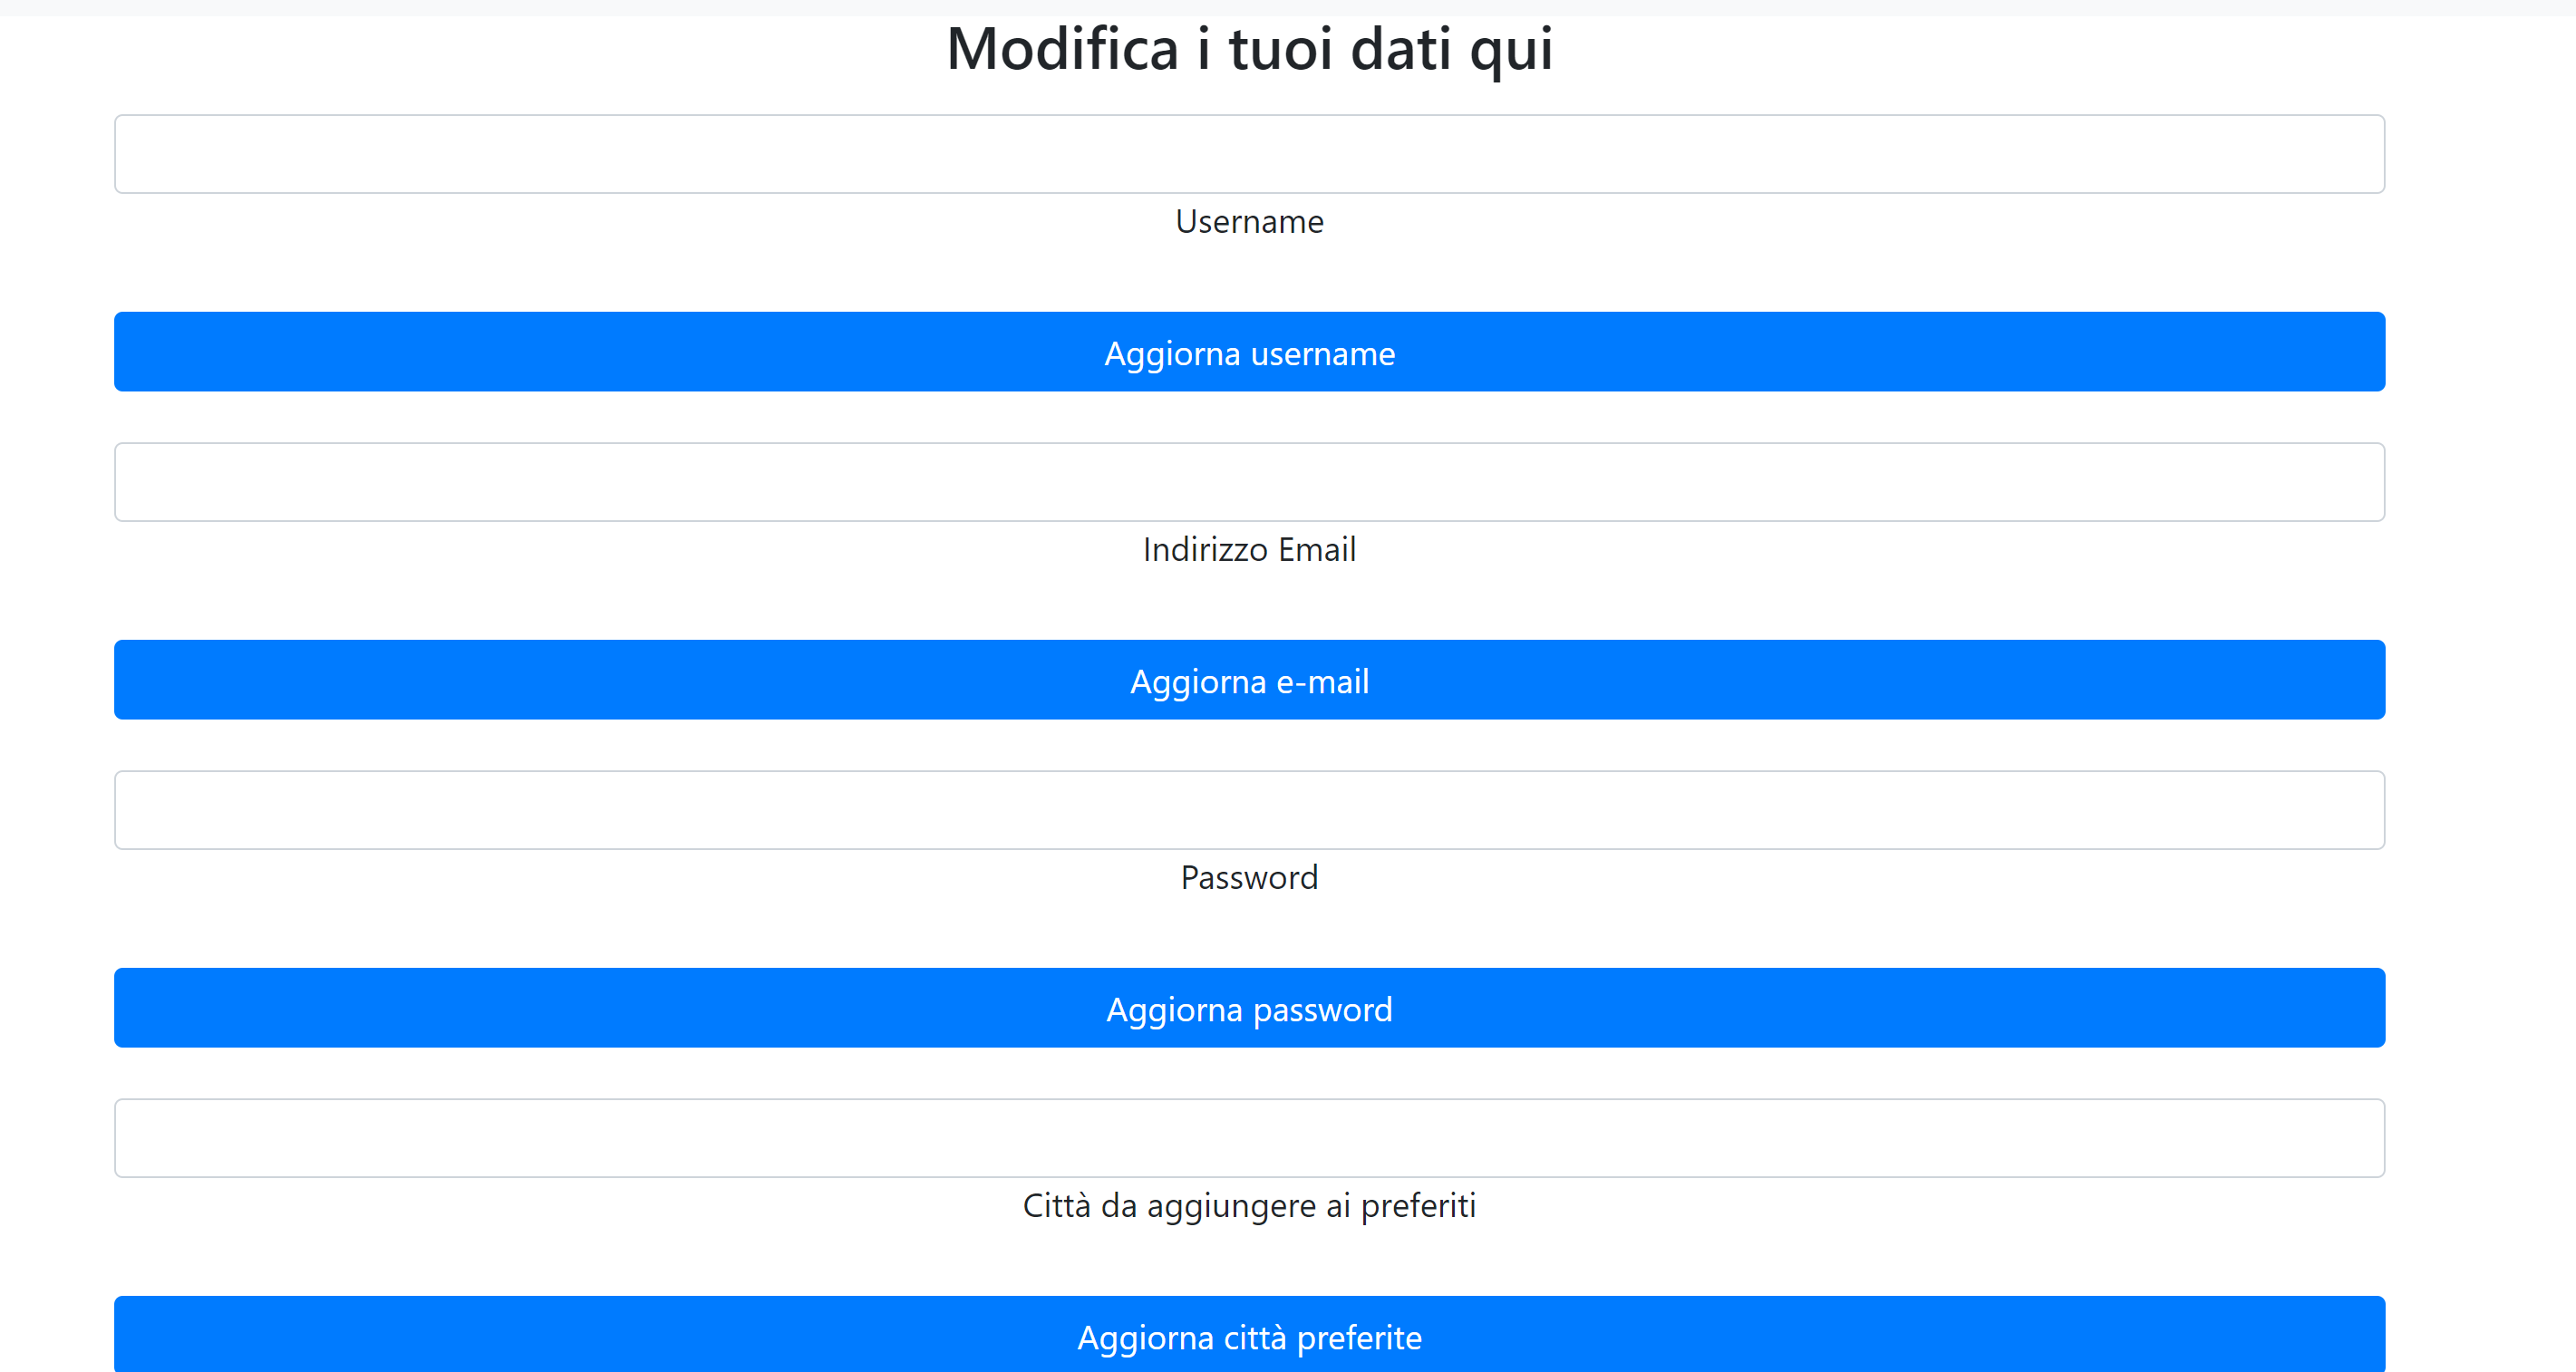
\includegraphics{img/areaPSotto.png}}
    \caption{Metà inferiore della pagina dedicata all'area personale}
\end{figure}

A seguito di queste informazioni, troviamo una serie di form che permettono, attraverso chiamate asincrone al server, di modificare
i dati relativi all'utente, quali:
\begin{itemize}
    \item username
    \item email
    \item password
    \item città salvate tra i preferiti
\end{itemize}